% !TEX TS-program = xelatex
\documentclass[12pt,letterpaper]{article}
\usepackage{amsmath,amssymb}
\usepackage{fontspec}
\setmainfont{EB Garamond}[Numbers=OldStyle,Ligatures=TeX]
\usepackage{tikz}
\usetikzlibrary{positioning,arrows.meta,fit,backgrounds,shapes.geometric}
\usepackage[letterpaper,margin=1in]{geometry}

\begin{document}

\section*{Option 1: Minimal DAG (6 nodes)}

\begin{figure}[h]
\centering
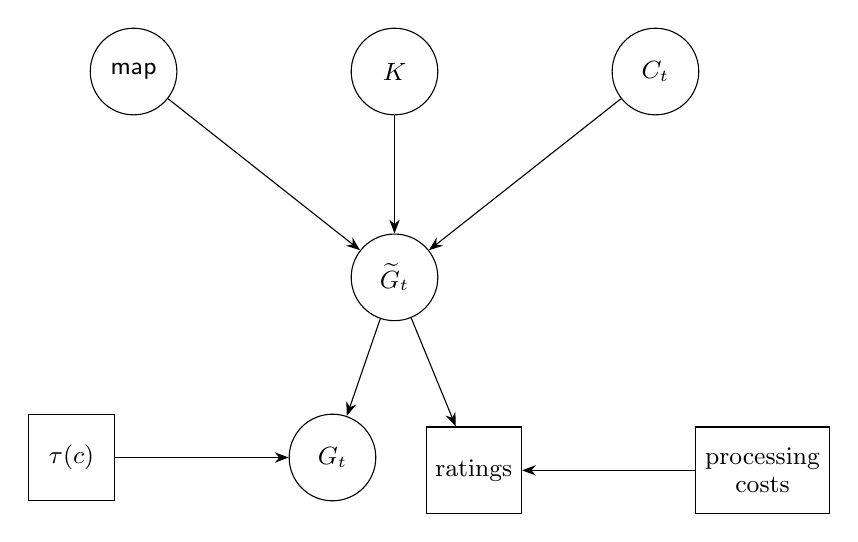
\begin{tikzpicture}[
  node distance=1.8cm and 2.2cm,
  latent/.style={draw,circle,minimum size=1.1cm,font=\small},
  observed/.style={draw,rectangle,minimum size=1.1cm,font=\small},
  every edge/.style={draw,-{Stealth[length=5pt]}},
]
  % State layer
  \node[latent] (map) {$\mathsf{map}$};
  \node[latent,right=of map] (K) {$K$};
  \node[latent,right=of K] (Ct) {$C_t$};

  % Stability score
  \node[latent,below=1.5cm of K] (Gtilde) {$\widetilde{G}_t$};

  % Membership
  \node[latent,below left=1.5cm and 0cm of Gtilde] (Gt) {$G_t$};
  \node[observed,left=of Gt] (tau) {$\tau(c)$};

  % Observation
  \node[observed,below right=1.5cm and 0cm of Gtilde] (ratings) {ratings};
  \node[observed,right=of ratings] (proc) {\shortstack{processing\\costs}};

  % Edges: state
  \path (map) edge (Gtilde);
  \path (K) edge (Gtilde);
  \path (Ct) edge (Gtilde);

  % Edges: threshold
  \path (Gtilde) edge (Gt);
  \path (tau) edge (Gt);

  % Edges: observation
  \path (Gtilde) edge (ratings);
  \path (proc) edge (ratings);
\end{tikzpicture}
\caption*{\textbf{Option 1: Minimal.} Circles = latent; rectangles = observed/set. Ratings reflect $\widetilde{G}_t$ plus processing costs, not $G_t$ directly.}
\end{figure}

\clearpage
\section*{Option 2: Medium DAG (11 nodes)}

\begin{figure}[h]
\centering
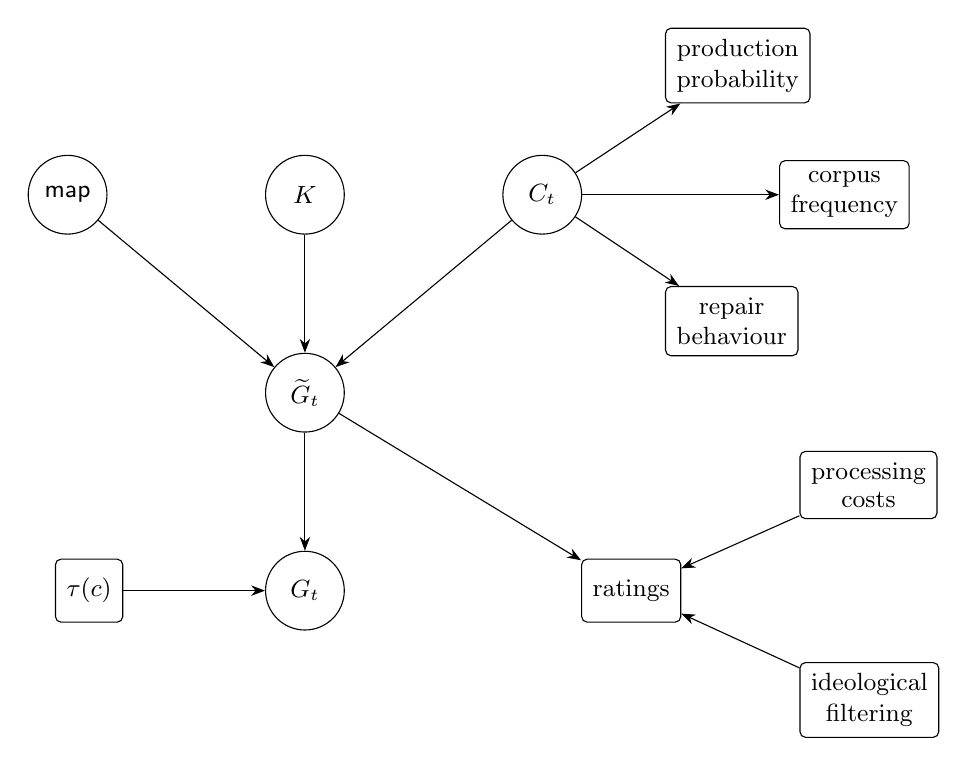
\begin{tikzpicture}[
  node distance=1.6cm and 2cm,
  latent/.style={draw,circle,minimum size=1cm,font=\small},
  observed/.style={draw,rectangle,rounded corners=2pt,minimum height=0.8cm,font=\small,inner sep=4pt},
  every edge/.style={draw,-{Stealth[length=5pt]}},
]
  % State layer
  \node[latent] (map) {$\mathsf{map}$};
  \node[latent,right=of map] (K) {$K$};
  \node[latent,right=of K] (Ct) {$C_t$};

  % Stability score
  \node[latent,below=1.5cm of K] (Gtilde) {$\widetilde{G}_t$};

  % Membership
  \node[latent,below=1.5cm of Gtilde] (Gt) {$G_t$};
  \node[observed,left=1.8cm of Gt] (tau) {$\tau(c)$};

  % Observation layer
  \node[observed,right=3cm of Gt] (ratings) {ratings};
  \node[observed,above right=0.5cm and 1.5cm of ratings] (proc) {\shortstack{processing\\costs}};
  \node[observed,below right=0.5cm and 1.5cm of ratings] (ideo) {\shortstack{ideological\\filtering}};

  % C_t indicators (above and right of C_t)
  \node[observed,above right=0.8cm and 1.2cm of Ct] (prod) {\shortstack{production\\probability}};
  \node[observed,right=2.5cm of Ct] (corpus) {\shortstack{corpus\\frequency}};
  \node[observed,below right=0.8cm and 1.2cm of Ct] (repair) {\shortstack{repair\\behaviour}};

  % Edges: state
  \path (map) edge (Gtilde);
  \path (K) edge (Gtilde);
  \path (Ct) edge (Gtilde);

  % Edges: threshold
  \path (Gtilde) edge (Gt);
  \path (tau) edge (Gt);

  % Edges: observation (from G̃_t, not G_t)
  \path (Gtilde) edge (ratings);
  \path (proc) edge (ratings);
  \path (ideo) edge (ratings);

  % Edges: C_t indicators (C_t causes the observations)
  \path (Ct) edge (prod);
  \path (Ct) edge (corpus);
  \path (Ct) edge (repair);
\end{tikzpicture}
\caption*{\textbf{Option 2: Medium.} Adds $C_t$'s observable indicators (right) and ideological filtering. $C_t$ is latent, inferred from converging evidence.}
\end{figure}

\clearpage
\section*{Option 3: Full DAG — polished}

\begin{figure}[h]
\centering
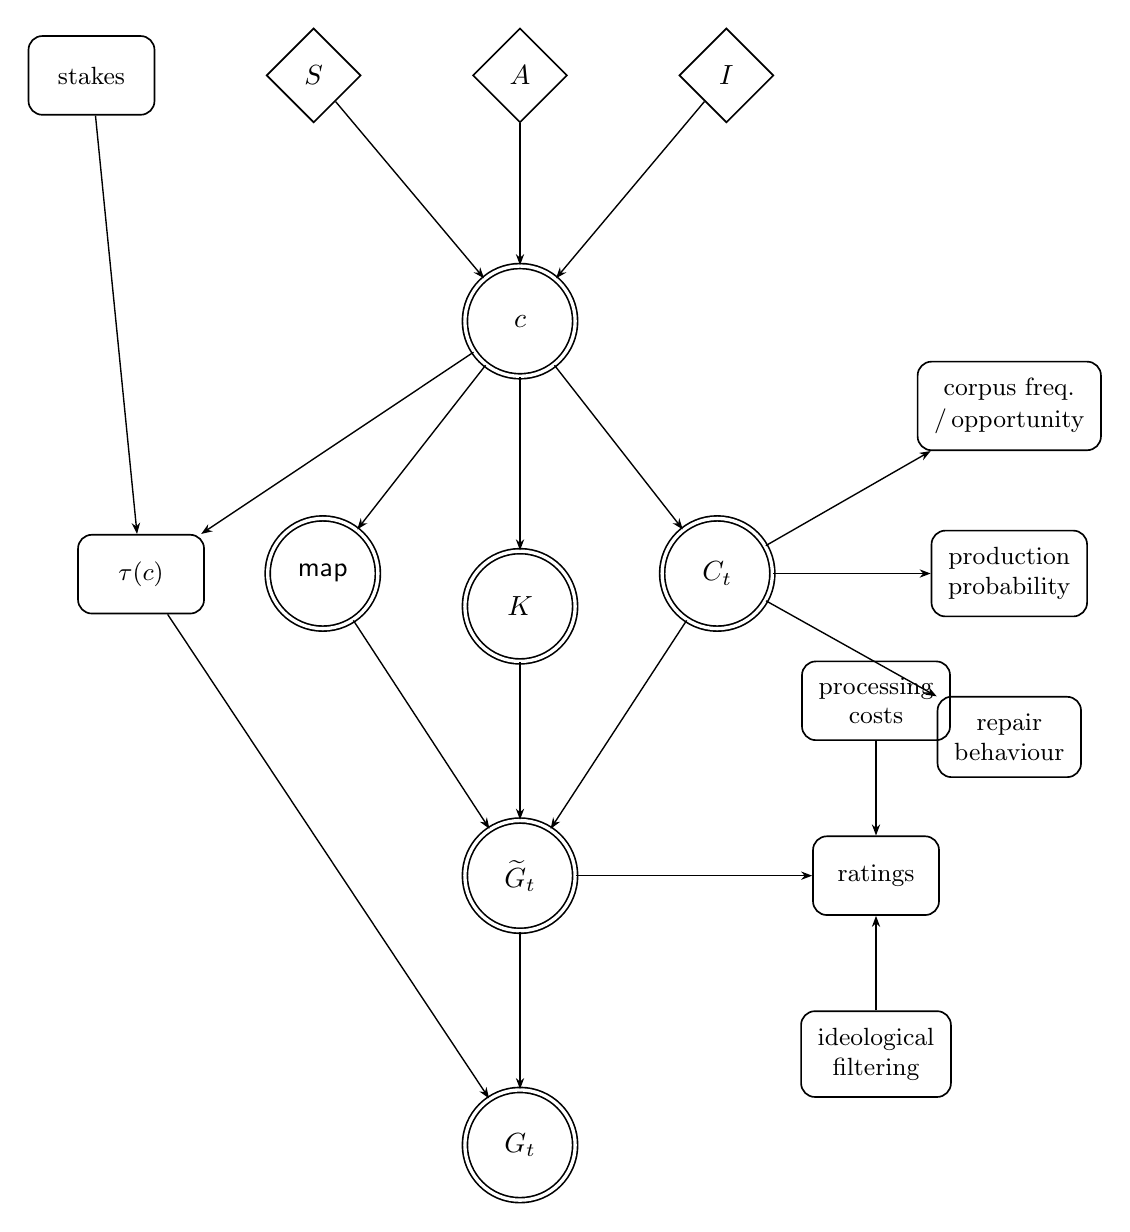
\begin{tikzpicture}[
  node distance=2cm and 1.8cm,
  % Double-stroke circles for latent variables
  latent/.style={circle, double, draw, double distance=1.2pt,
    line width=0.6pt, minimum size=1.4cm, font=\normalsize,
    inner sep=0pt},
  % Rounded rectangles for observed/set quantities
  observed/.style={rectangle, rounded corners=5pt, draw,
    line width=0.6pt, minimum height=1cm, minimum width=1.6cm,
    font=\small, inner sep=6pt},
  % Larger diamonds for conditioning anchors
  cond/.style={diamond, draw, line width=0.6pt, minimum size=1.2cm,
    font=\normalsize, inner sep=3pt},
  % Thin arrows with small heads
  every edge/.style={draw, line width=0.5pt, -{Stealth[length=4pt, width=3pt]}},
]
  % === Layer 1: Conditioning ===
  \node[observed] (stakes) {stakes};
  \node[cond,right=1.4cm of stakes] (S) {$S$};
  \node[cond,right=1.4cm of S] (A) {$A$};
  \node[cond,right=1.4cm of A] (I) {$I$};

  % === c node ===
  \node[latent,below=1.8cm of A] (c) {$c$};

  % === Layer 2: State variables + threshold ===
  \node[observed,below left=2.2cm and 3.5cm of c] (tau) {$\tau(c)$};
  \node[latent,below left=2.2cm and 1.5cm of c] (map) {$\mathsf{map}$};
  \node[latent,below=2.2cm of c] (K) {$K$};
  \node[latent,below right=2.2cm and 1.5cm of c] (Ct) {$C_t$};

  % === Layer 3: Stability score ===
  \node[latent,below=2cm of K] (Gtilde) {$\widetilde{G}_t$};

  % === Layer 4: Membership ===
  \node[latent,below=2cm of Gtilde] (Gt) {$G_t$};

  % === Observation branch (right, from G̃_t) ===
  \node[observed,right=3cm of Gtilde] (ratings) {ratings};
  \node[observed,above=1.2cm of ratings] (proc) {\shortstack{processing\\costs}};
  \node[observed,below=1.2cm of ratings] (ideo) {\shortstack{ideological\\filtering}};

  % === C_t indicators (right, from C_t directly) ===
  \node[observed,right=2cm of Ct] (prod) {\shortstack{production\\probability}};
  \node[observed,above=1cm of prod] (corpus) {\shortstack{corpus freq.\\/\,opportunity}};
  \node[observed,below=1cm of prod] (repair) {\shortstack{repair\\behaviour}};

  % === Edges: conditioning ===
  \path (S) edge (c);
  \path (A) edge (c);
  \path (I) edge (c);
  \path (stakes) edge (tau);
  \path (c) edge (tau);

  % === Edges: c → state variables ===
  \path (c) edge (map);
  \path (c) edge (K);
  \path (c) edge (Ct);

  % === Edges: state → stability ===
  \path (map) edge (Gtilde);
  \path (K) edge (Gtilde);
  \path (Ct) edge (Gtilde);

  % === Edges: threshold → membership ===
  \path (Gtilde) edge (Gt);
  \path (tau) edge (Gt);

  % === Edges: observation (from G̃_t, NOT G_t) ===
  \path (Gtilde) edge (ratings);
  \path (proc) edge (ratings);
  \path (ideo) edge (ratings);

  % === Edges: C_t → indicators (all direct from C_t) ===
  \path (Ct) edge (prod);
  \path (Ct) edge (corpus);
  \path (Ct) edge (repair);
\end{tikzpicture}
\caption*{\textbf{Option 3 (polished).} Circles (double-stroke)\,=\,latent; rounded rectangles\,=\,observed/set; diamonds\,=\,conditioning anchors. Ratings are downstream of $\widetilde{G}_t$ (stability), not $G_t$ (membership). $C_t$ indicators are each direct outputs of $C_t$.}
\end{figure}

\end{document}
